\begin{frame}
\frametitle{Installation}
\begin{itemize}
\item Download from \url{https://www.python.org/}
\item For Ubuntu download from repository:\lstinputlisting[language=bash, firstline=1, lastline=1, numbers=none]{./install-commands.txt}

\item For Windows, download from \url{https://www.python.org/downloads/windows/}

\item For Ubuntu installing packages:\lstinputlisting[language=bash, firstline=2, lastline=2, numbers=none]{./install-commands.txt}

\item For Windows installing packages if $C:\backslash Python\backslash Scripts \backslash$ is in the path:\lstinputlisting[language=bash, firstline=3, lastline=3, numbers=none]{./install-commands.txt}

\item For Windows installing packages:\lstinputlisting[language=bash, firstline=4, lastline=4, numbers=none]{./install-commands.txt}
\end{itemize}
\end{frame}

\begin{frame}
\frametitle{Introduction}
\begin{itemize}
\item For Windows, the default editer is IDLE
\begin{figure}
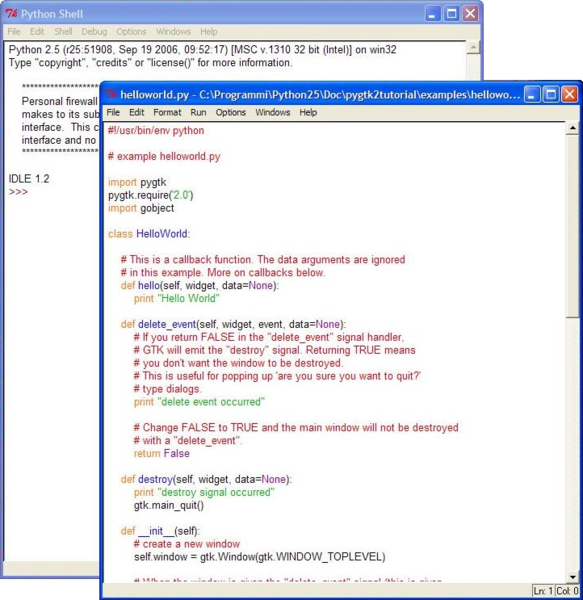
\includegraphics[width=0.8\linewidth, height=0.5\linewidth]{idle.png}
\end{figure}
\end{itemize}
\end{frame}

